\documentclass[11pt,a4paper]{article}

\usepackage{blindtext}
\usepackage[T1]{fontenc}
\usepackage[utf8]{inputenc}
\usepackage{amsmath}
\usepackage{setspace}
\usepackage{underscore}
\usepackage{geometry}
\usepackage{bbm}
\usepackage{hyperref}
\usepackage[title]{appendix}
\usepackage{mathrsfs}
\hypersetup{hidelinks,
	colorlinks=true,
	allcolors=black,
	pdfstartview=Fit,
	breaklinks=true}
\usepackage[table,xcdraw]{xcolor}
\usepackage{enumerate,authblk,indentfirst,authblk,ragged2e}
\usepackage{graphicx}
\usepackage{float}
\usepackage{subfigure} 
\usepackage{cite}
\usepackage{comment}
\setlength{\parskip}{0.5em} 
\setlength{\parindent}{2em} 
\geometry{a4paper,left=1.8cm,right=1.8cm,top=2cm,bottom=2.1cm}

\begin{document}
%{\tiny {\tiny {\scriptsize {\scriptsize {\tiny }}}}}
%\title{Forecasting Shanghai Second-hand House Price}
\begin{center}
\huge\textbf{Forecasting Shanghai Second-hand House Price}
\large\textbf{Group 11 \\
Chen Taoyue 1155141543  \\
DAI Qiyu 1155141616\\
JIANG Yunhui 1155141677 \\
LI Linyuan 1155141569 \\
MAK Man Fung 1155141893 \\
QIN Zihao 1155124920 }
%{\tiny {\tiny {\scriptsize {\scriptsize {\tiny }}}}}
\date{}
\end{center}
\tableofcontents
%\author{Group 11 \\
%Chen Taoyue 1155141543  \\
%DAI Qiyu 1155141616\\
%JIANG Yunhui 1155141677 \\
%LI Linyuan 1155141569 \\
%MAK Man Fung 1155141893 \\
%QIN Zihao 1155124920 }
%\maketitle
%\tableofcontents
\thispagestyle{empty}
\newpage
	%\maketitle
	\doublespacing
	\setcounter{page}{1}
	\section{Introduction} 
    In developed Chinese cities, the property price is crucial to all potential and existing holders. According to an official article posted by YUNXIOK \footnote{YUNXINOK: https://www.yun-xk.com/details/fj/930.html}, the price of Shanghai's property is volatile, which has soared three times in the past two decades but slumped this year. Also, most of the apartments transacted in Shanghai are second-hand apartments, whose price is more unpredictable than that of new flats. Such fluctuating patterns in property prices and the lack of information hurt the stability of buyers and sellers and increase the difficulty for government to regulate.
	
	On the other hand, thanks to the advancement in information technology, the availability of big data on housing information is tremendously increased. More importantly, we are able to invoke modern machine-learning techniques in data mining. Thus motivated, this project aims to convey insights into the Shanghai property market via a data-driven approach from two perspectives: 
	\begin{itemize}
	  \item Forecasting the price of pre-owned properties by regression models.
    \item Identifying factors that influence the price significantly.
	\end{itemize}

	The remainder of this report is organized as follows. We first answer questions on where our data comes from and how to process it in Section 2. Then, section 3 presents the model-building approaches. Several important determinants of house price are emphasized in Section 4, and Section 5 concludes. Additional plots and numerical results are contained in Appendix.

    \section{Data}
    \subsection{Data Description}
    This project uses python to automatically collect the pre-owned apartments' information from the website of \href{https://sh.lianjia.com/ershoufang}{\textit{Lianjia}},which is the largest online property agency in mainland China. The reasons for using such a data source are twofold. Firstly, it can provide us with a rich-data environment. After dropping the irrelevant columns, there are still 21,299 records, each described by a long vector of 22 features. For a detailed explanation of the variables, please check Appendix 6.1. Secondly, the dataset is more up-to-date than off-the-shelf data on websites like Kaggle since it is collected at the beginning of this project. Thus, real-time updates of housing information in Shanghai are included. Combined, our project can adequately reflect the underlying pattern of the current housing market.
    
    \subsection{Data Splitting and Visualization}
    The acquired dataset is randomly divided into two parts, with $80\%$ training data and 20$\%$ testing data. We calculate the model parameters with training data, and then assess the model performance in the testing sample. 
    
    Before data pre-processing, we first visualize the training dataset to gain insights. Firstly, looking at the density curve for the price, it is observed that the distribution is right-skewed. Hence, a log transformation is conducted. We also compare the boxplots before and after taking the log. As shown in Figure 1 (refer to Appendix 6.2), the log transformation significantly reduces the number of outliers, which leads us to expect that it can improve the fitting of models.
    
    \subsection{Data Cleaning}
   Upon closely examining our dataset, we find that it contains information on two categories, with 15 columns containing categorical features and 7 columns including numerical attributes.

   To deal with textual categorical features, We first filter out trivial characters. Then dummy encoding is employed to convert each categorical feature with n levels into (n-1) dummy variables. Furthermore, numerical variables are extracted by string manipulation functions. For instance, for contents like "five bedrooms two parlous one kitchen two toilets" in Chinese, four corresponding values could be obtained as features of the apartments' layout. After the above procedure, the data sample has 75 dimensions total, with 63 dummies and 12 numerical variables.     


\subsection{Data Transformation}
We then computed the proportion of missing data for each column. The number of missing data is reasonably small or even zero for most features, which indicates the good quality of our data. Nevertheless, to avoid a waste of information, we decide to utilize the k-nearest neighbors algorithm to impute missing data instead of directly discarding them. 

A suite of different $k$ is compared in order to prevent our imputation strategy from hurting model prediction performance. That is, we feed the training data into a pipeline consisting of an imputer and a random forest regressor. Then, following the philosophy of cross-validation, the prediction error for a grid hyperparameters is recorded. Given the mean and standard deviation of negative RMSE across different folds for each $k$, 33 is selected. After plugging in the optimal number of neighbors, a KNN imputer is calculated on all training data and then applied to the testing set. 

Also, we observe that the scales of numerical features differ significantly, which may impact the models' sensitivity to outliers. Therefore, standardization is required to address the problem. Similar to imputation, we normalize the whole dataset using the mean and standard deviation of the training set.
 
At the end of data pre-processing, an additional visualization step is conducted. By projecting all inputs on a three-dimensional scatter plot using principal component analysis (PCA), a crucial information is gained. As displayed in Appendix 6.2, Figure 2, our data is well-separated looking from different angles. Hence, the upcoming models are expected to perform well.
    \section{Model Building}
    \subsection{Overall Workflow}
Before diving into the core part of this section, we first overview the workflow comprised of three stages. Firstly, we select the model with an optimal level of complexity using a grid search with five-fold cross-validation. Then, the full training data is employed for fitting. Lastly, we evaluate the models' performance on new data points using a testing set.

When choosing the model parameters, the parameter candidate sequence is adjusted until the chosen value lies in the middle of the set rather than the boundary. Additionally, considering the huge volume of the dataset, we allow Python to run all computer processors in a parallel manner for acceleration.

In order to assess the goodness of models, three metrics are employed: R-squared, root-mean-squared-error (RMSE), and mean-absolute error (MAE). R-squared represents the proportion of variance for the dependent variable explained by the model. RMSE and MAE quantify how deviated the model prediction is from the truth. Moreover, they share the same units as the target variable and thus have an intuitive meaning. Let $\hat{y}$ and $y$ be the estimate and true value of the forecasting target; their mathematical definitions are  \\
\centerline{$R^2=\frac{\sum_{i=1}^N (\hat{y}-\bar{\hat{y}})^2}{\sum_{i=1}^N(y-\bar{y})^2}$, $MSE=\sqrt{\sum_{i=1}^N (\hat{y}-y)^2}$, $MAE=\sum_{i=1}^N |\hat{y}-y|$}

    \subsection{Models}
    \begin{enumerate}
        \item \textbf{OLS and Penalized Regression}  \\
        The starting point of our model construction efforts is ordinary least squares (OLS) regression. It has the benefits of being both computationally efficient and simple to understand. However, the fitting performance of both in-sample and out-of-sample is not unsatisfactory, with an R-squared around $85\%$. Clearly, the reason is its inflexibility since linear restrictions are imposed.
        
        It should be mentioned that people usually include penalized regression in machine learning projects as a common practice. However, given the current situation, we don't bother to discuss them in detail. From a theoretical point of view, the difference in OLS training and testing fitting is insignificant, implying that imposing regularization on coefficients will not help too much; empirically, as illustrated in Appendix 6.3, table 1, the advantages of LASSO, RIDGE, and Elastic Net are not obvious in terms of forecasting the testing set. Moreover, almost no parameters are shrunk exactly to zero for LASSO, meaning the interpretability is low.
        \item \textbf{SVR}  \\
        The first model for dealing with the large bias of OLS prediction is Support Vector Machine Regressor (SVR). The objective of SVR is to find a hyperplane with most instances around it as the decision boundary. Furthermore, the kernel function could be applied to implement its non-linear structure. The best kernel is selected to be Radial Basis Function using five-fold cross-validation, and the results of the tuned model show that the high bias has been alleviated to some extent.
        \item \textbf{KNN}  \\
        Furthermore, the k-nearest neighbors (KNN) algorithm is carried out to boost the in-sample fitting performance, considering the flexibility due to its non-parametric nature. 
        This intelligent method works by directly computing the weighted mean of the k nearest neighbors for a new point.
        Two crucial parameters, $k$ and the weighting scheme, are again pinned down by cross-validation. Notably, the selected $k$ given by 1, which causes perfect in-sample fitting. However, the error on testing data is even larger than that of OLS, implying the considerable variance of such a complex model.
        \item \textbf{Decision Tree}  \\
        We then applied tree-based methods, which are among the most popular approaches in machine learning. A decision tree is implemented by doing recursive binary partitions. By default, the package in python tends to split the data until only pure leaf nodes are left, causing the instability of model prediction errors. Therefore, we similarly conducted a grid search to determine the depth and other tree properties.
        
        Regarding the results of the decision tree, there are two key remarks. Firstly, though tuning parameters are carefully chosen, the gap between training and testing accuracy is still remarkable. Such a high variance issue should be tackled. Secondly, there is still room for reducing in-sample error, which is attributed to the bias of the model. Being aware of these limitations, ensemble learning methods are further developed afterward.
        \item \textbf{Random Forest} \\
       We first utilize a random forest algorithm to handle the overfitting problem of the decision tree. There, each tree is constructed independently on a bootstrap sample of input points and by selecting a random subset of all features. As for making forecasts, a data point will be passed by multiple trees, and the final decision is made by taking the average.
        
Given the above bagging (bootstrap and aggregation) mechanism, random forest is hard to encounter overfitting. Therefore, tuning the depth of the tree will not be that rewarding, and we simply set it to be the optimal value of the decision tree (30). The grid search is performed on two parameters, the number of features used in each tree and the number of trees in the whole forest. From Table 1 in Appendix, random forest mitigated the overfitting problem and increased out-of-sample R-square.
\item \textbf{Boosting} \\
Additionally, we experiment with three boosting algorithms. Unlike random forests, which grow multiple trees independently, boosting algorithm's implementation is sequential. Specifically, the Ada boosting regressor grows the next tree while assigning higher weights to instances with larger errors in the previous step. As for gradient boosting, it adds a new decision tree that best reduces the loss function before. Furthermore, compared with gradient boosting, the extension of XGB lies in the regularization of the estimation procedure, which controls overfitting. 

After choosing the optimal learning rate and other parameters using grid search, it is found that the Ada and XGB boosting perform well, with an R-squared over $91\%$ on the testing set. However, gradient boosting overfits a bit.
    \end{enumerate}
 Table 1 in Appendix 6.3 summarizes the overall performance of all models. After comparison, we claim that random forest, Ada boosting, and XGB boosting outperform the other methods. Thus, in the next section, we compute the importance of features based on these three models as they have superb prediction ability.
 \section{Variable Importance}
 In this project, feature importance could be interpreted as predictive power. Moreover, in the tree model context, it is measured by the improvement in the split criterion. Notice that if a feature participates in multiple nodes, an average should be taken.

Several most important variables are reviewed here. On the one hand, random forest and Ada boosting agree that area$\_$size and inner are the two most essential predictors. On the other hand, XGB boosting ranks office and Chongming at the top. One possible reason why XGB holds a distinct view from the other two might be its regularization, which leads to a different objective function and/or additional constraints. Additionally, notice that area$\_$size is a numerical variable, and the remaining four are dummies. Specifically, inner indicates whether a house is located in the inner string of Shanghai; office refers to places with commercial use instead of residential purpose; Chongming and Jianshan are names of districts. A more comprehensive comparison can be seen in Appendix 6.2, Figure 3.
\section{Conclusion}
In summary, we scrapped an updated and large dataset from the Lianjia website. After conducting data-pre-processing, the performance of the difference estimation method in predicting Shanghai housing prices is evaluated. Based on the results, we recommend three algorithms with excellent out-of-sample performance, which are Random Forest, Ada boosting and XGB boosting. Finally, the most important variables were pointed out. 

With the information provided in this project, buyers and sellers of properties in Shanghai will benefit from the mitigated difficulties of assessing apartment prices. Also, our model is worth being used as a reference by the government and private institutions like consulting firms and equity research companies when studying Shanghai real estate market issues.
 
Nevertheless, we note that there are two main caveats to our analysis. Firstly, information from the \href{https://sh.lianjia.com/ershoufang}{\textit{Lianjia}} website like apartment reviews is not incorporated. These types of textual data require deep learning methods to process, which, unfortunately, are beyond the course scope. Secondly, out of \href{https://sh.lianjia.com/ershoufang}{\textit{Lianjia}} website, factors such as government regulation and economic environment should also be taken into consideration. It is hoped that these limitations will be circumvented in the future.


\newpage
\section{Appendix}
\subsection{Data description}
\begin{figure}[H]
    \centering
    \subfigure[Data Description]
    {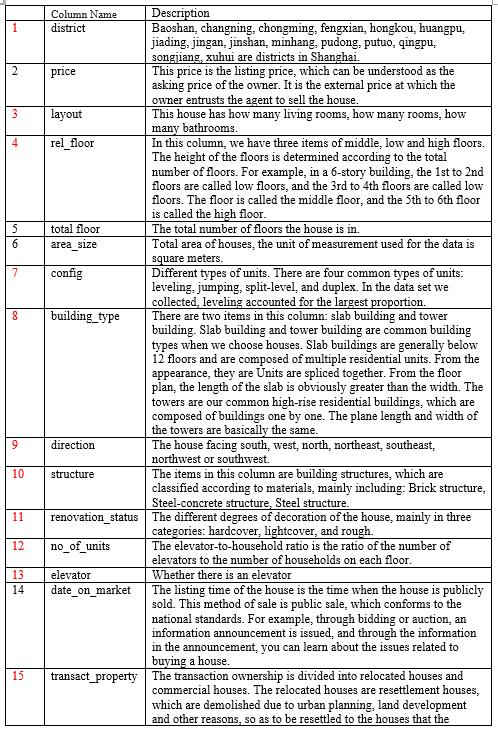
\includegraphics[width=17cm,height=23cm]{../../figures/21.jpg}}
    \end{figure}
\begin{figure}[H]
    \subfigure[Data Description]
    {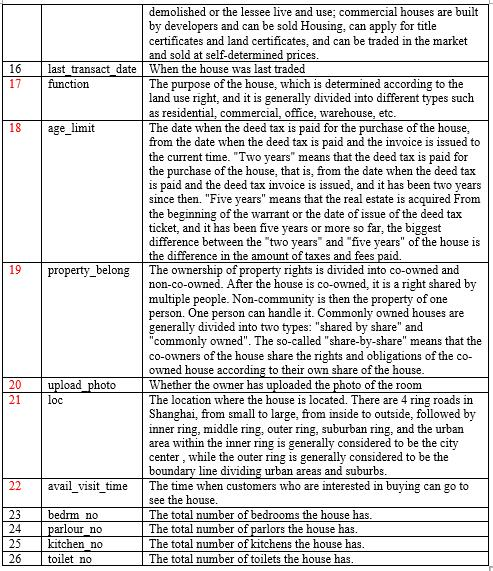
\includegraphics[width=17cm]{../../figures/22.jpg}}
    \end{figure}
The serial numbers of some columns are marked in red, indicating that they are categorical features and will be transformed to dummy variables after data processing.

\subsection{Visualization}
 \begin{figure}[H]
    \centering
    \subfigure[Before Log-Transformation]{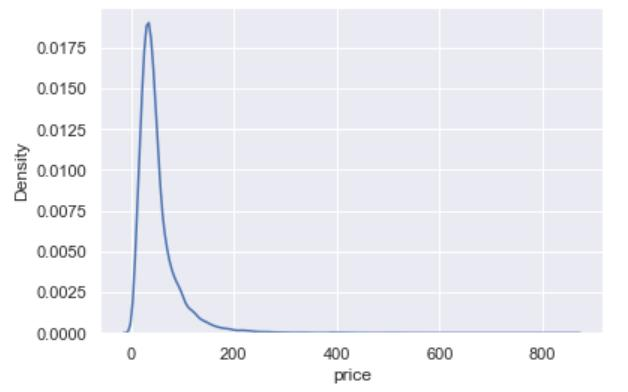
\includegraphics[width=8cm]{../../figures/before density.jpg}}
    \subfigure[After Log-Transformation]{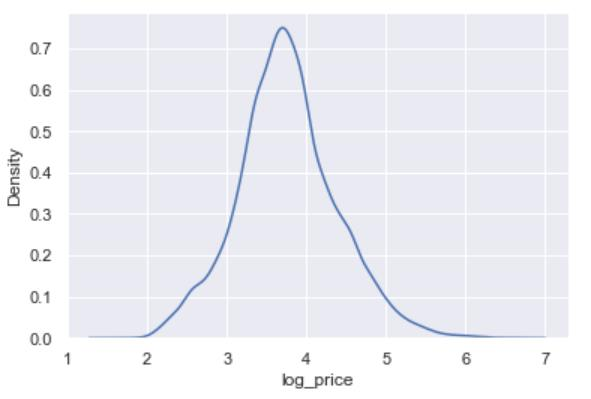
\includegraphics[width=7.5cm]{../../figures/after density.jpg}}
    \subfigure[Before Log-Transformation]{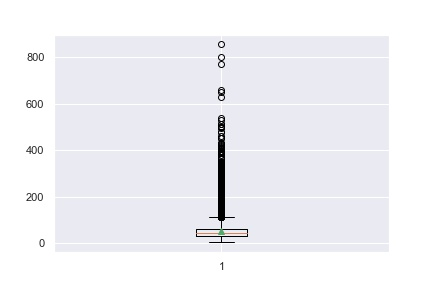
\includegraphics[width=8cm]{../../figures/before plot.jpg}}
    \subfigure[After Log-Transformation]{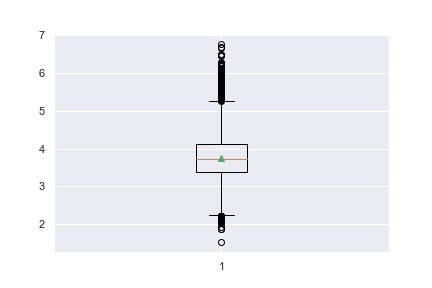
\includegraphics[width=8cm]{../../figures/after plot.jpg}}
    \caption{Density plot of price and Bloxplot of Price}
\end{figure}

\begin{figure}[H]
    \centering
    {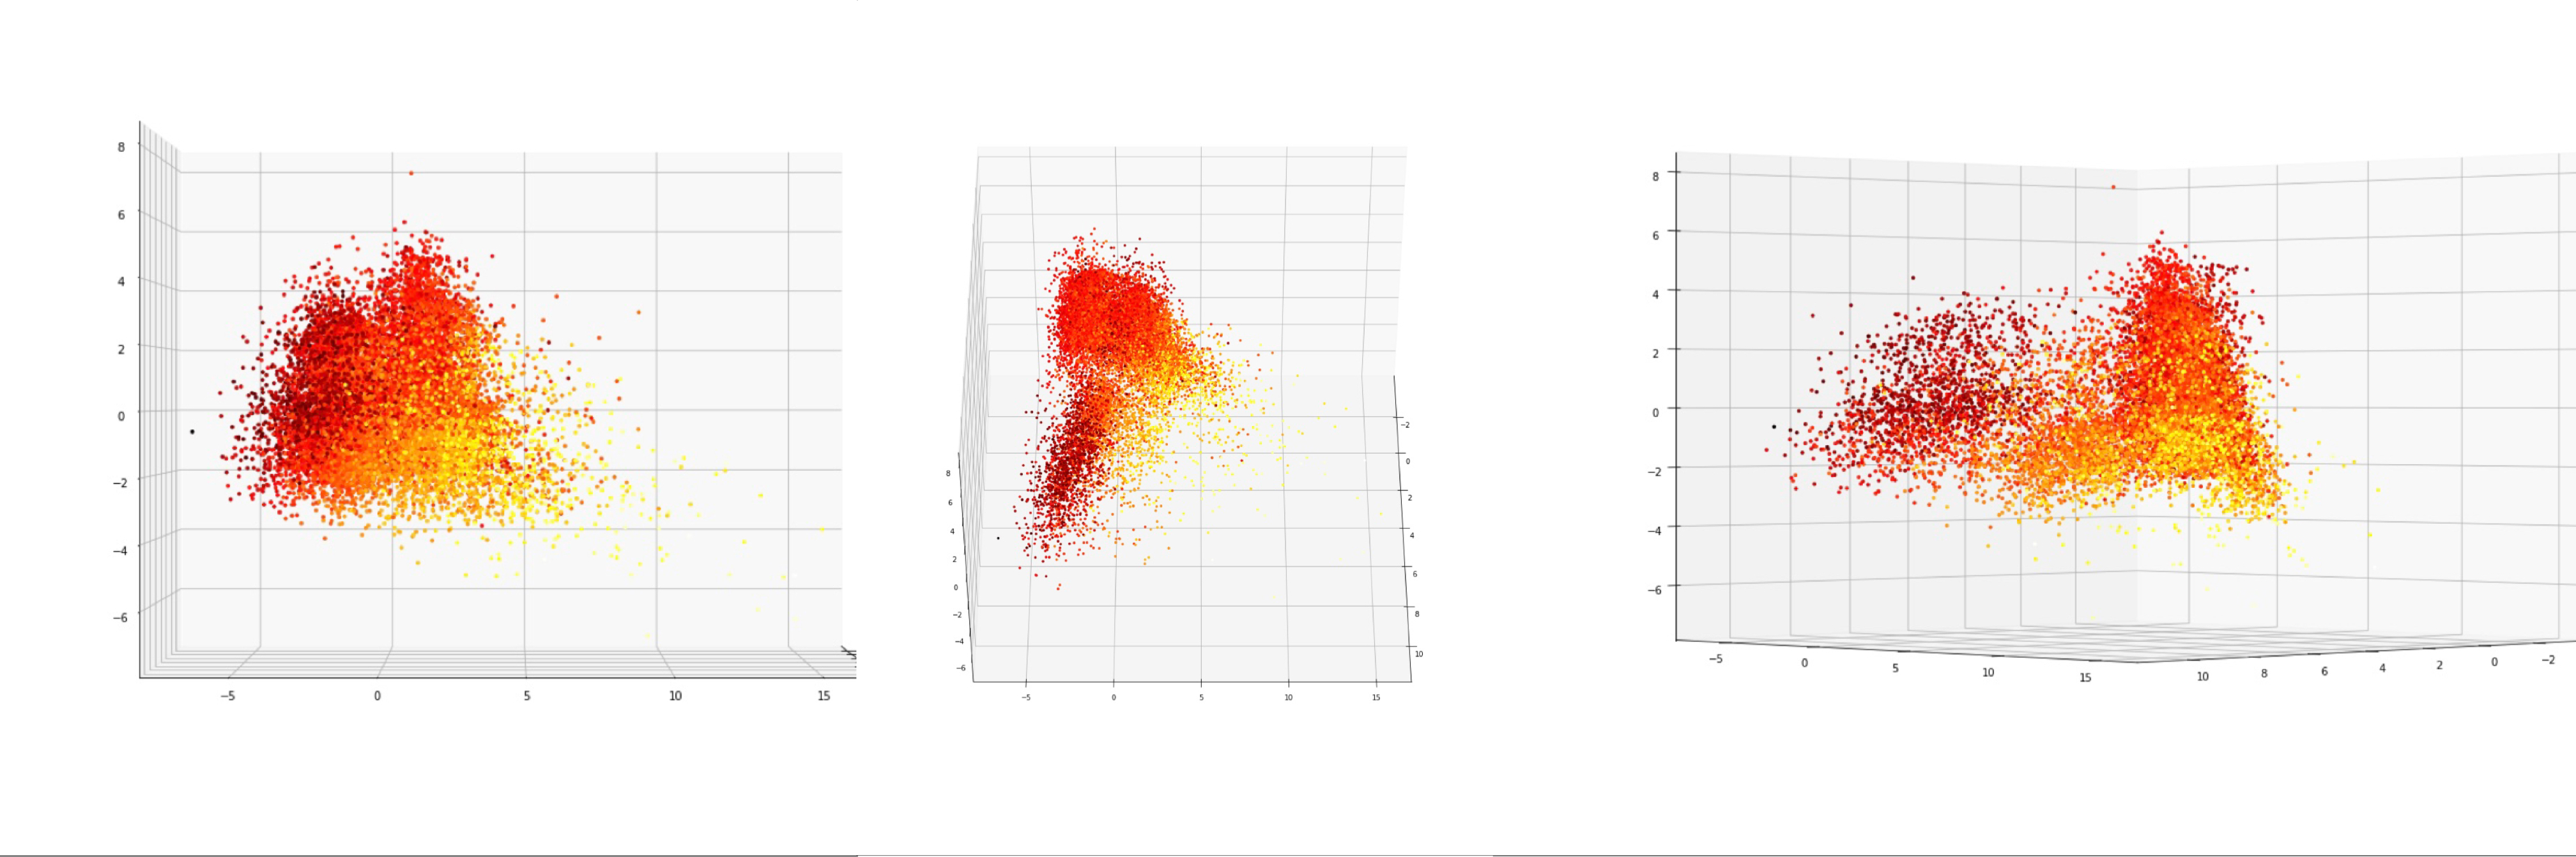
\includegraphics[width=18cm]{../../figures/pca.jpg}}
    \caption{principal component analysis}
\end{figure}

\begin{figure}[H]
    \centering
    \subfigure[Ada boosting]{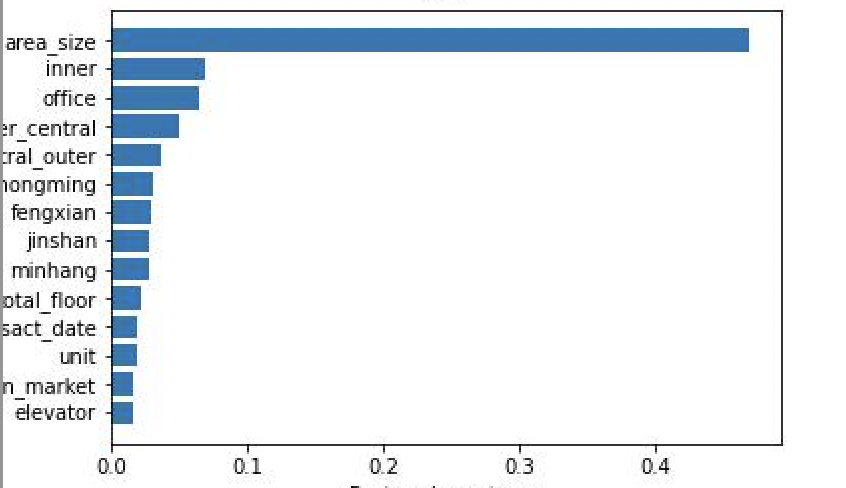
\includegraphics[width=5.5cm,height=3cm]{../../figures/ada.png}}
    \subfigure[XGB boosting]{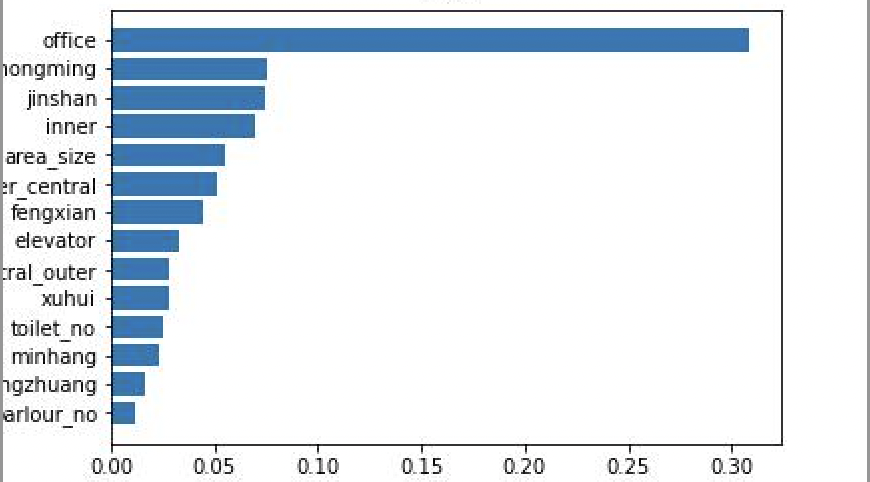
\includegraphics[width=5.5cm]{../../figures/xgb.png}}
    \subfigure[Random Forest]{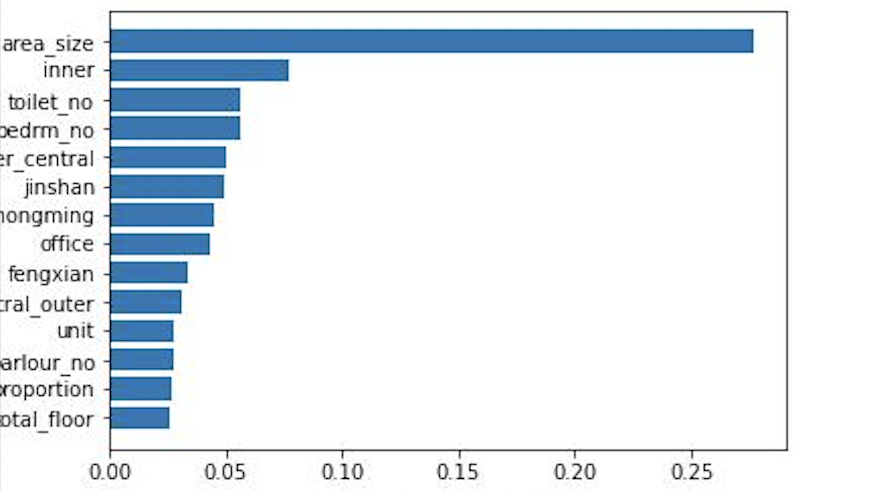
\includegraphics[width=5.5cm]{../../figures/rfr.png}}
    \caption{Feature Importance}
\end{figure}

\subsection{Result}
\begin{table}[H]
\centering
\begin{tabular}{|c|cc|cc|cc|}
\hline
\textbf{}                                     & \multicolumn{2}{c|}{\textbf{R-squared}}                                                                                      & \multicolumn{2}{c|}{\textbf{RMSE}}                                                                                           & \multicolumn{2}{c|}{\textbf{MAE}}                                                                                            \\ \hline
\textbf{}                                     & \multicolumn{1}{c|}{\textbf{training}}                                              & \textbf{testing}                       & \multicolumn{1}{c|}{\textbf{training}}                                              & \textbf{testing}                       & \multicolumn{1}{c|}{\textbf{training}}                                              & \textbf{testing}                       \\ \hline
\textbf{OLS}                                  & \multicolumn{1}{c|}{\textbf{0.8516}}                                                & \textbf{0.8450}                        & \multicolumn{1}{c|}{{\color[HTML]{24292F} \textbf{0.2476}}}                         & {\color[HTML]{24292F} \textbf{0.2557}} & \multicolumn{1}{c|}{{\color[HTML]{24292F} \textbf{0.1886}}}                         & {\color[HTML]{24292F} \textbf{0.1948}} \\ \hline
\textbf{Lasso}                                & \multicolumn{1}{c|}{\textbf{0.8515}}                                                & \textbf{0.8455}                        & \multicolumn{1}{c|}{\textbf{0.2476}}                                                & \textbf{0.2554}                        & \multicolumn{1}{c|}{\textbf{0.1886}}                                                & \textbf{0.1946}                        \\ \hline
\textbf{Ridge}                                & \multicolumn{1}{c|}{\textbf{0.8516}}                                                & \textbf{0.8454}                        & \multicolumn{1}{c|}{\textbf{0.2476}}                                                & \textbf{0.2554}                        & \multicolumn{1}{c|}{\textbf{0.1886}}                                                & \textbf{0.1946}                        \\ \hline
\textbf{Elastic\_net}                         & \multicolumn{1}{c|}{{\color[HTML]{24292F} \textbf{0.8454}}}                         & {\color[HTML]{24292F} \textbf{0.8365}} & \multicolumn{1}{c|}{{\color[HTML]{24292F} \textbf{0.2527}}}                         & {\color[HTML]{24292F} \textbf{0.2627}} & \multicolumn{1}{c|}{{\color[HTML]{24292F} \textbf{0.1891}}}                         & {\color[HTML]{24292F} \textbf{0.1962}} \\ \hline
\textbf{KNN}                                  & \multicolumn{1}{c|}{{\color[HTML]{24292F} \textbf{1}}}                              & {\color[HTML]{24292F} \textbf{0.7901}} & \multicolumn{1}{c|}{{\color[HTML]{24292F} \textbf{0.0}}}                            & {\color[HTML]{24292F} \textbf{0.2976}} & \multicolumn{1}{c|}{{\color[HTML]{24292F} \textbf{0.0}}}                            & {\color[HTML]{24292F} \textbf{0.2271}} \\ \hline
\textbf{SVR}                                  & \multicolumn{1}{c|}{{\color[HTML]{24292F} \textbf{0.9429}}}                         & {\color[HTML]{24292F} \textbf{0.8888}} & \multicolumn{1}{c|}{{\color[HTML]{24292F} \textbf{0.1535}}}                         & {\color[HTML]{24292F} \textbf{0.2166}} & \multicolumn{1}{c|}{{\color[HTML]{24292F} \textbf{0.1134}}}                         & {\color[HTML]{24292F} \textbf{0.1541}} \\ \hline
\textbf{Decision Tree}                        & \multicolumn{1}{c|}{{\color[HTML]{24292F} \textbf{0.9206}}}                         & {\color[HTML]{24292F} \textbf{0.8741}} & \multicolumn{1}{c|}{{\color[HTML]{24292F} \textbf{0.1811}}}                         & {\color[HTML]{24292F} \textbf{0.2305}} & \multicolumn{1}{c|}{{\color[HTML]{24292F} \textbf{0.137}}}                          & {\color[HTML]{24292F} \textbf{0.1679}} \\ \hline
\rowcolor[HTML]{B6D7A8} 
{\color[HTML]{CC0000} \textbf{Random Forest}} & \multicolumn{1}{c|}{\cellcolor[HTML]{B6D7A8}{\color[HTML]{CC0000} \textbf{0.9892}}} & {\color[HTML]{CC0000} \textbf{0.9172}} & \multicolumn{1}{c|}{\cellcolor[HTML]{B6D7A8}{\color[HTML]{CC0000} \textbf{0.0667}}} & {\color[HTML]{CC0000} \textbf{0.187}}  & \multicolumn{1}{c|}{\cellcolor[HTML]{B6D7A8}{\color[HTML]{CC0000} \textbf{0.0484}}} & {\color[HTML]{CC0000} \textbf{0.1345}} \\ \hline
\rowcolor[HTML]{B6D7A8} 
{\color[HTML]{CC0000} \textbf{Ada boosting}}  & \multicolumn{1}{c|}{\cellcolor[HTML]{B6D7A8}{\color[HTML]{CC0000} \textbf{0.9998}}} & {\color[HTML]{CC0000} \textbf{0.9191}} & \multicolumn{1}{c|}{\cellcolor[HTML]{B6D7A8}{\color[HTML]{CC0000} \textbf{0.0101}}} & {\color[HTML]{CC0000} \textbf{0.1848}} & \multicolumn{1}{c|}{\cellcolor[HTML]{B6D7A8}{\color[HTML]{CC0000} \textbf{0.0029}}} & {\color[HTML]{CC0000} \textbf{0.1269}} \\ \hline
\textbf{Grandient boosting}                   & \multicolumn{1}{c|}{{\color[HTML]{24292F} \textbf{0.9954}}}                         & {\color[HTML]{24292F} \textbf{0.8584}} & \multicolumn{1}{c|}{{\color[HTML]{24292F} \textbf{0.0436}}}                         & {\color[HTML]{24292F} \textbf{0.2445}} & \multicolumn{1}{c|}{{\color[HTML]{24292F} \textbf{0.0336}}}                         & {\color[HTML]{24292F} \textbf{0.1709}} \\ \hline
\rowcolor[HTML]{B6D7A8} 
{\color[HTML]{CC0000} \textbf{XGB boosting}}  & \multicolumn{1}{c|}{\cellcolor[HTML]{B6D7A8}{\color[HTML]{CC0000} \textbf{0.9867}}} & {\color[HTML]{CC0000} \textbf{0.9197}} & \multicolumn{1}{c|}{\cellcolor[HTML]{B6D7A8}{\color[HTML]{CC0000} \textbf{0.0742}}} & {\color[HTML]{CC0000} \textbf{0.1841}} & \multicolumn{1}{c|}{\cellcolor[HTML]{B6D7A8}{\color[HTML]{CC0000} \textbf{0.0584}}} & {\color[HTML]{CC0000} \textbf{0.1334}} \\ \hline
\end{tabular}
\caption{Overall results}
\label{tab:my-table}
\end{table}
\end{document} 
